\item \textbf{{[}YIJC/PRELIM/9569/2020/P1/Q7{]} }

The College\textquoteright s local area network (LAN) is connected
to the MOE Headquarter\textquoteright s LAN over the internet. 
\begin{center}
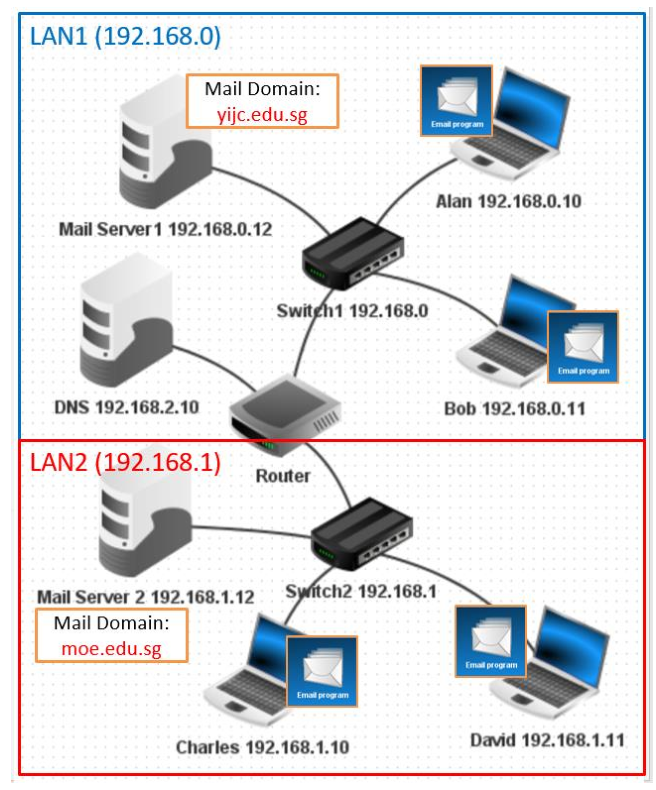
\includegraphics[width=0.5\paperwidth]{C:/Users/Admin/Desktop/Github/question_bank/LyX/static/img/9569-YIJC-2020-P1-Q7}
\par\end{center}

A staff in the college, Alan, sends an email to Charles who works
in the MOE Headquarter.
\begin{enumerate}
\item The following questions should take reference from the above network
diagram. 
\begin{enumerate}
\item Describe the function of the Domain Name System (DNS) server.\hfill{}
{[}1{]}
\item Explain how the router identifies that the MOE's Mail server is residing
in another network.\hfill{} {[}1{]}
\item Describe in detail how Alan's email is delivered and kept in the MOE's
Mail server.\hfill{} {[}2{]}
\item Describe how Charles eventually receive Alan\textquoteright s email.\hfill{}
{[}2{]}
\end{enumerate}
\item Charles forwards Alan\textquoteright s email to his colleague, David.
Describe how David could receive the email even when he is away from
the office. \hfill{}{[}2{]}
\end{enumerate}